\documentclass[aps, pra, superscriptaddress, reprint, floatfix]{revtex4-2}

\usepackage{graphicx}   % For including graphics
\usepackage[colorlinks = true, linkcolor=teal, citecolor=teal, urlcolor  = teal]{hyperref}
\usepackage{algorithm}  % For algorithm environment
\usepackage{algpseudocode}  % For algorithmic environment
\usepackage{amsmath}    % For amsmath features
\usepackage{amssymb}    % For amssymb features
\usepackage{color}
\usepackage{physics}
\usepackage{tikz}
\usepackage{dsfont}
\usepackage{booktabs}
\usepackage{times}
\usepackage{comment}


\usepackage[capitalize]{cleveref}
\usepackage{quantikz}
\usepackage{svg}

\usetikzlibrary{shapes.geometric}
\usepackage{relsize}
\usepackage{tcolorbox}
\usepackage{enumerate}
\usepackage{amsthm}
\usepackage{orcidlink}

\crefname{equation}{Eq.}{equations}
\crefname{section}{Sec.}{sections}
\crefname{figure}{Fig.}{figures}
\crefname{appendix}{Appendix}{appendices}
\crefname{table}{Table}{tables}

\theoremstyle{plain}
\newtheorem{theorem}{Theorem}
\newtheorem{lemma}[theorem]{Lemma}
\newtheorem{proposition}[theorem]{Proposition}
\newtheorem{remark}[theorem]{Remark}
\newtheorem{corollary}[theorem]{Corollary}
\AfterEndEnvironment{theorem}{\noindent\ignorespaces}
\AfterEndEnvironment{lemma}{\noindent\ignorespaces}
\AfterEndEnvironment{corollary}{\noindent\ignorespaces}

\newtheorem{definition}[theorem]{Definition}
\AfterEndEnvironment{definition}{\noindent\ignorespaces}
\AfterEndEnvironment{proof}{\noindent\ignorespaces}

\newcommand{\je}[1]{\textcolor{cyan}{#1}}
\newcommand{\as}[1]{\textcolor{orange}{#1}}
\newcommand{\mf}[1]{\textcolor{violet}{#1}}
\newcommand{\SC}[1]{\textcolor{pink}{#1}}
\newcommand{\equalcontrib}{These authors contributed equally.}

\newcommand{\mc}{\mathcal}
\newcommand{\bs}{\boldsymbol}
\newcommand*\diff{\mathop{}\!\mathrm{d}}
\newcommand{\REF}{\textcolor{red}{![REF]!}}

\DeclareMathOperator*{\argmin}{arg\,min}

\begin{document}

\title{Computational regimes in matrix-product-state-based quantum trajectory simulations}

\author{Aaron Sander\,\orcidlink{0009-0007-9166-6113}}
\affiliation{Technical University of Munich, Munich, Germany}

\author{Simon Cichy}
\affiliation{Freie Universität Berlin, Berlin, Germany}

\author{Martin Eigel\,\orcidlink{0000-0003-2687-4497}}
\affiliation{Weierstrass Institute for Applied Analysis and Stochastics, Berlin, Germany}

\author{Jens Eisert\,\orcidlink{0000-0003-3033-1292}}
\affiliation{Freie Universität Berlin, Berlin, Germany}
\affiliation{Helmholtz-Zentrum Berlin für Materialien und Energie, Berlin, Germany}

\author{Maximilian Fröhlich\,\orcidlink{0009-0007-5276-2858}}
\affiliation{Weierstrass Institute for Applied Analysis and Stochastics, Berlin, Germany}

\author{Tom Peham\,\orcidlink{0000-0003-3434-7881}}
\affiliation{Technical University of Munich, Munich, Germany}

\author{Robert Wille\,\orcidlink{0000-0002-4993-7860}}
\affiliation{Technical University of Munich, Munich, Germany}
\affiliation{Munich Quantum Software Company GmbH, Munich, Germany}
\affiliation{Software Competence Center Hagenberg GmbH (SCCH), Hagenberg, Austria}

\date{\today}

\begin{abstract}
Efficient simulation of open quantum systems is central to modeling noisy quantum hardware and many-body dynamics. In trajectory-based tensor network methods, cost is often associated with trajectory-level quantities such as entanglement growth or bond dimension. However, the total cost of a fixed-accuracy simulation also depends on statistical sampling, and the interplay between per-trajectory complexity and sampling effort remains poorly understood. Here we introduce a cost-resolved framework for matrix product state (MPS)-based quantum trajectory simulations that decomposes total cost into memory per trajectory, runtime per trajectory, and sampling effort. We show that physically equivalent stochastic unravelings of the same Lindblad dynamics do not necessarily reduce total cost, but instead redistribute cost between trajectory complexity and statistical convergence. This trade-off is quantified by two dimensionless inflation factors: a bond dimension inflation $\alpha$ and a sampling inflation $\kappa$, which together determine the preferred unraveling under hardware-dependent memory and parallelism constraints. We provide a practical protocol for extracting $(\alpha,\kappa)$ from modest pilot simulations and demonstrate it using benchmarks across multiple noise channels. The resulting decision maps show that the computationally favorable unraveling can change with noise strength, time-step resolution, system size, and available parallelism. These results establish unraveling choice as a hardware-aware simulation design problem rather than an intrinsic optimization of trajectory entanglement alone.
\end{abstract}

\maketitle

\section{Introduction}
The accurate simulation of open quantum systems constitutes a central challenge in quantum science, underpinning the modeling and validation of noisy quantum devices, many-body dynamics, and near-term quantum algorithms. This perspective is grounded in the fundamental observation that every quantum system is, to some extent, open and inevitably interacts with its environment.
In the context of quantum computing, noise represents a principal obstacle. It is therefore crucial not only to understand in detail how quantum noise affects coherent dynamics, but also to delineate the regimes of quantum evolution that can be effectively ``dequantized'' through 
advanced classical simulation techniques \cite{Zhou_2020}. Over the past decade, applying advanced classical simulation methods to quantum simulation platforms of steadily increasing capability has proven to be a highly fruitful endeavor \cite{Zhou_2020,PRXQuantum.5.010308,Trotzky}: This helps assessing the computational power of quantum simulators and to turn paradigmatic settings into quantum technological devices \cite{MindTheGaps}.
In such efforts, tensor network methods take center stage. Indeed, in many-body settings, tensor network methods---most prominently \emph{matrix product state} (MPS) techniques for one spatial dimension---provide a scalable classical 
framework by exploiting the typically limited entanglement structure of 
relevant quantum states~\cite{White1992, vidal_2004, Schollwock_2011,AreaReview,
RevModPhys.93.045003,Orus-AnnPhys-2014}. For closed systems, the computational cost of MPS simulations is closely tied to entanglement growth, as captured by the bond dimension.

Among possible model descriptions, Markovian or Lindbladian open quantum systems are particularly important. They capture forgetful quantum dynamics, which is ubiquitous for weakly
coupled quantum systems and appears naturally in many physical settings. Open system dynamics governed by Lindblad master equations can be simulated using trajectory-based approaches, which unravel the mixed state evolution into ensembles of stochastic pure state trajectories~\cite{Dalibard_1992, Molmer_92, Carmichael_1993, Wiseman_Milburn_2009}. In MPS-based implementations, each stochastic trajectory is represented as an individual many-body pure state whose time evolution is sampled repeatedly to reconstruct physical observables. The computational object of interest is therefore not the density matrix itself, but the ensemble of stochastic trajectories that approximate it. Consequently, the relevant notion of entanglement for assessing trajectory-level simulation complexity is that of the individual trajectories rather than that of the mixed state generated by the Lindblad dynamics.

A substantial body of work has investigated how specific stochastic unravelings and measurement-induced dynamics influence entanglement along individual trajectories. In particular, continuous monitoring schemes and suitably chosen unravelings can significantly suppress trajectory entanglement or alter its scaling behavior~\cite{block_2022, liu_2024, cecile_2024, guimaraes_2023, leung_2024, kshetrimayum_2017}. More recently, Vovk and Pichler have systematically explored the freedom inherent in stochastic unravelings, introducing 
entanglement-optimized and conventional schemes and demonstrating that unraveling choice can qualitatively reshape trajectory entanglement scaling, including finite-size transitions between area- and volume-law behavior and exponential cost separations between MPS trajectories and \emph{matrix product operator} (MPO)-based simulations in specific models~\cite{vovk_2022, vovk_2024}.
A rigorous underpinning of entanglement-optimal mixed state decompositions has been delivered in Ref.\
\cite{SimonSimulation}. These results and rigorous insights establish that unraveling choice can dramatically modify trajectory entanglement properties, suggesting that apparent simulation cost may depend sensitively on how the master equation is decomposed.

The present work shifts the focus from entanglement scaling to end-to-end computational cost. Rather than asking only how unravelings modify trajectory entanglement, we ask how trajectory-level properties translate into total runtime under fixed-accuracy requirements and realistic hardware constraints. In large-scale simulations, computational effort is not governed by a single diagnostic but is distributed across distinct cost channels. Trajectory-based methods incur memory costs set by the bond dimension of individual trajectories, runtime costs determined by both bond dimension and numerical resolution, and stochastic sampling costs associated with the number of trajectories required for convergence. While each of these contributions has been discussed in prior work~\cite{daley_2014, transchel_2014, weimer_2021, moroder_2023,SimonSimulation}, their combined impact on total runtime at scale has, to the best of our knowledge, not been analyzed within a unified, cost-resolved framework.

In this work, we introduce a cost-resolved framework for analyzing computational complexity in MPS-based quantum trajectory simulations. Rather than ranking unravelings or seeking universally optimal schemes, we ask how physical noise parameters, numerical choices, and hardware constraints redistribute computational effort at fixed accuracy. Separating memory, runtime, and sampling contributions leads to two dimensionless inflation factors, $(\alpha,\kappa)$, which define a decision geometry for comparing physically equivalent unravelings under finite memory and parallelism. We also provide a practical protocol for extracting these factors from modest pilot simulations.

To reach system sizes beyond exact state-vector methods, we employ the \emph{tensor jump method} (TJM), a trajectory formulation of Lindblad dynamics that evolves ensembles of MPS pure states and avoids the exponential overhead of density-matrix simulation~\cite{sander_TJM_2025}. Here, TJM serves as a scalable benchmarking platform for studying how trajectory bond dimension, stochastic sampling, and finite computational resources jointly determine simulation cost~\cite{daley_2014, transchel_2014, weimer_2021, moroder_2023, zwolak_2004}. We benchmark one-dimensional spin models with local depolarizing noise up to 80 sites and complement these results with Heisenberg-model case studies under additional noise channels.

Our results show that reduced trajectory bond dimension does not automatically translate into reduced end-to-end simulation cost. Entanglement suppression can be offset by increased sampling requirements or by the need for finer time-step resolution. The preferred unraveling is therefore not an intrinsic property of the Lindblad model alone, but depends on how per-trajectory complexity, statistical convergence, and available hardware resources combine. In particular, strategies favored on memory-limited architectures may differ from those favored on highly parallel hardware.

\section{Quantum trajectory simulations}
This section introduces the theoretical and algorithmic framework underlying quantum trajectory simulations of open quantum systems. We summarize the Lindblad formalism, its stochastic unravelings, and the numerical parameters that control trajectory evolution. No assumptions about computational cost or scaling behavior are being made at this stage.

\subsection{Lindblad dynamics and quantum trajectories}
The interaction of a quantum system with a weakly coupled, memoryless environment is commonly modeled by a Lindblad master equation~\cite{Lindblad1976, Breuer_2007}. Let $\rho \in \mathcal{B}(\mathcal{H})$ denote the system density operator and $H_0 \in \mathcal{B}(\mathcal{H})$ the closed system Hamiltonian acting on a Hilbert space $\mathcal{H}$. The Lindblad equation reads
\begin{equation}
\label{eq:Lindblad}
\frac{d}{dt}\rho
= -i[H_0,\rho]
+ \sum_{m=1}^k \gamma_m
\left(
L_m \rho L_m^\dagger
- \frac{1}{2}\{L_m^\dagger L_m, \rho\}
\right),
\end{equation}
where $\{L_m\}_{m=1}^k \subset \mathcal{B}(\mathcal{H})$ are jump operators describing dissipative processes such as relaxation, excitation, or dephasing, and $\{\gamma_m\}_{m=1}^k$ are the corresponding non-negative dissipation rates.

The direct integration of Eq.~\eqref{eq:Lindblad} is, however, generally computationally intractable  
already for moderately sized quantum systems, i.e., it scales exponentially with system size due to the dimension of $\rho \in \mathbb{C}^{d^L \times d^L}$ where $d$ is the physical dimension and $L$ is the system size.
Trajectory-based approaches avoid this bottleneck by unraveling the Lindblad dynamics into ensembles of stochastic pure state trajectories~\cite{Dalibard_1992, Carmichael_1993, Molmer_92, Wiseman_Milburn_2009}. Physical observables are recovered by averaging over trajectories.

In the specific \emph{Monte Carlo wavefunction} (MCWF) formalism, each trajectory evolves under an effective non-Hermitian Hamiltonian
\begin{equation}
\label{eq:Heff}
H = H_0 - \frac{i}{2}\sum_{m=1}^k \gamma_m L_m^\dagger L_m,
\end{equation}
interrupted by stochastic quantum jumps. Over a time step $\delta t$, the 
state vector evolves according to
\begin{equation}
\ket{\Psi(t+\delta t)} = e^{-iH\delta t}\ket{\Psi(t)},
\end{equation}
with a total jump probability
\begin{equation}
\delta p(t)
= \sum_{m=1}^k \delta t\, \gamma_m
\langle \Psi(t) | L_m^\dagger L_m | \Psi(t) \rangle.
\end{equation}
If a jump occurs, a jump operator $L_m$ is applied with probability proportional to its contribution to $\delta p(t)$, otherwise, the state vector is renormalized. Repeating this procedure generates a stochastic trajectory $\ket{\Psi_j(t)}$. Ensemble 
averages approximate expectation values,
\begin{equation}
\langle O(t) \rangle
= \frac{1}{N}\sum_{j=1}^N
\bra{\Psi_j(t)} O \ket{\Psi_j(t)} ,
\end{equation}
with statistical convergence governed by standard Monte Carlo sampling, i.e., $\mathcal{O}(1/\sqrt{N})$ with a variance-dependent pre-factor, as a faithful estimator for the mixed quantum state at time $t$.

\subsection{Unraveling freedom}
The stochastic representation of Lindblad dynamics is not unique. A given Lindblad equation admits infinitely many stochastic unravelings, corresponding to different ways of resolving environmental interactions at the level of individual trajectories~\cite{Wiseman_Milburn_2009}. While all valid unravelings reproduce the same mixed state dynamics upon ensemble averaging, they generally generate distinct trajectory ensembles.

From a physical perspective, different unravelings are commonly associated with different measurement or monitoring schemes applied to the environment, such as quantum jump, diffusive, or hybrid descriptions~\cite{Wiseman_Milburn_2009, daley_2014}. This freedom has been extensively explored in the context of measurement-induced dynamics and monitoring-driven entanglement phenomena, where unraveling choice strongly affects trajectory-level properties~\cite{block_2022, liu_2024, guimaraes_2023, leung_2024}.

The freedom in choosing stochastic unravelings reflects the non-uniqueness of the Lindblad operator decomposition, i.e., different sets of jump operators and associated monitoring schemes generate distinct ensembles of pure state trajectories while reproducing the same mixed state evolution. Vovk and 
Pichler have systematically explored this freedom, demonstrating that appropriately chosen unravelings can alter trajectory entanglement scaling and even induce finite-size transitions between area- and volume-law behavior~\cite{vovk_2022, vovk_2024,AreaReview}.
Here, rather than seeking entanglement-minimizing unravelings, we treat this as a computational degree of freedom and analyze how different choices redistribute cost across bond dimension, runtime, and sampling requirements.

Although different unravelings reproduce the same Lindblad dynamics at the ensemble level, in the sense that they all give rise to faithful estimators of the quantum state at a given time, they are implemented in practice through concrete choices of dissipation rates, time step discretization, and stochastic update rules. A clear distinction between physical parameters and numerical control parameters is therefore crucial before their computational implications can be meaningfully addressed.

\subsection{Physical and numerical parameters}
Quantum trajectory simulations are governed by both physical and numerical parameters that control how the continuous-time Lindblad dynamics is realized algorithmically.
The dissipation rates $\{\gamma_m\}_{m=1}^k$ appearing in Eq.~\eqref{eq:Lindblad} are physical parameters fixed by the model. They determine the strength and relative weight of different noise channels and fully specify the Lindblad dynamics~\cite{Lindblad1976, Breuer_2007}.
The time step $\delta t$ is a numerical parameter that controls the temporal discretization of the stochastic evolution. In trajectory-based simulations, $\delta t$ sets both the resolution of the numerical integrator and the frequency with which the system is sampled for quantum jumps~\cite{Wiseman_Milburn_2009, daley_2014}. Different choices of $\delta t$ converge to the same physical dynamics in expectation, with discretization error $\mathcal{O}(\delta t^p)$ for $(p+1)$-order Trotterization, but can produce different stochastic realizations at the trajectory level.
The effective jump probability
\begin{equation}
\delta p \propto \gamma\, \delta t
\end{equation}
provides an emergent algorithmic measure of stochasticity per time step, up to state-dependent expectation values of the jump operators. Unlike $\gamma$, which is a physical parameter, or $\delta t$, which is numerical, $\delta p$ is not an independent control parameter but reflects their combined effect. In practice, $\delta p$ is frequently used as a heuristic proxy for noise strength in trajectory simulations. However, as we analyze explicitly in this work, $\delta p$ does not uniquely characterize trajectory behavior across different discretizations, even when ensemble dynamics coincide.

\subsection{Tensor network representation of trajectories}
Trajectory methods replace the exponential complexity of density matrix evolution by an approximate ensemble of pure states, reducing the memory scaling from $\mathcal{O}(d^{2L})$ to $\mathcal{O}(N d^L)$.
For large systems, this scaling remains prohibitive and motivates the use of tensor network representations for individual trajectories.
In one spatial dimension, state vectors $\ket{\Psi} \in \mathbb{C}^{d^L}$ can be efficiently represented as  \emph{matrix product state} (MPS) vectors~\cite{White1992, Vidal_2003, Schollwock_2011},
\begin{equation}
\ket{\Psi}
= \sum_{\sigma_1,\ldots,\sigma_L}
M^{\sigma_1}_1 \cdots M^{\sigma_L}_L
\ket{\sigma_1,\ldots,\sigma_L},
\end{equation}
where $M^{\sigma_\ell}_\ell \in \mathbb{C}^{\chi_{\ell-1} \times \chi_\ell}$ are local tensors and $\{\chi_\ell\}$ are bond dimensions encoding bipartite entanglement with boundaries $\chi_0=\chi_L=1$. When entanglement remains moderate, this representation yields polynomial scaling in system size with memory cost $\mathcal{O}(d L \chi^2)$ for a single trajectory. 
The computational cost of evolving an MPS typically scales with a higher power of the bond dimension, commonly as $\mathcal{O}(\chi^3)$ per local update, reflecting the cost of tensor contractions and local linear algebra, with the precise pre-factor depending on the chosen time-evolution scheme \cite{Schollwock_2011, Paeckel_2019}.

In this work, we employ the \emph{tensor jump method} (TJM)~\cite{sander_TJM_2025}, which combines stochastic quantum trajectories with matrix product state representations and \emph{time-dependent variational principle} (TDVP) evolution~\cite{Haegeman2011, Haegeman_2016, Paeckel_2019}. Between stochastic jump events, the state is propagated within the MPS manifold using TDVP, while quantum jumps are implemented as local operator insertions followed by canonicalization and controlled truncation. This structure enables large ensembles of trajectory simulations while maintaining a transparent separation between physical dynamics and numerical approximation.

The framework of quantum trajectories together with an MPS representation introduces a concrete set of resource controls. The bond dimension $\chi$ governs the memory footprint of individual trajectories and the cost of local tensor network updates, while the number of trajectories $N$ governs statistical convergence. In addition, the time step $\delta t$ controls how many updates are required to reach a fixed physical evolution time. These ingredients allow us to formalize the end-to-end computational cost of trajectory simulations in terms of distinct cost channels.
With the simulation ingredients fixed, we now turn from representation to resource accounting.


\section{Computational cost structure}
\label{sec:cost_structure}
Given an MPS representation of trajectories, the computational cost of a fixed-accuracy simulation is not governed by a single parameter. Instead, it separates into three distinct contributions: per-trajectory memory cost, per-trajectory runtime cost, and sampling cost, the latter reducible through parallel execution of independent trajectories.

To compare physically equivalent stochastic unravelings within this multi-channel structure, we introduce two dimensionless ratios, a bond dimension inflation factor $\alpha$, capturing relative per-trajectory memory and runtime scaling, and a sampling inflation factor $\kappa$, quantifying relative sampling effort at fixed accuracy. We then derive a hardware-aware criterion that determines which unraveling is favored under given memory and parallelism constraints.

In practice, MPS-based trajectory simulations approximate the exact Lindblad dynamics through a combination of finite time-step integration, projection onto a finite-bond dimension variational manifold, and finite stochastic sampling. Throughout this work, ``fixed accuracy'' means convergence with respect to the numerical controls relevant for the comparison, e.g., the time step $\delta t$, the MPS truncation criterion, and the statistical uncertainty of the trajectory estimator. For large systems, where exact reference evolution is unavailable, the sampling component refers to the estimated standard error of the trajectory average rather than a directly measured absolute error to the exact Lindblad solution.

\subsection{Three canonical cost channels}
We consider trajectory-based simulations in which expectation values are estimated from an ensemble of $N$ independent trajectories, each represented as an MPS with characteristic maximum bond dimension $\chi$. The total cost then consists of the following components:
\begin{enumerate}
\item {\textbf{Per-trajectory memory cost (MPS storage).}}
For a one-dimensional MPS, the memory footprint of a single trajectory scales as
\begin{equation}
\mathrm{mem}(\chi) \propto L\, d\, \chi^2,
\label{eq:mem_scaling_def}
\end{equation}
up to implementation-dependent constants~\cite{Schollwock_2011}.

\item{\textbf{Per-trajectory runtime cost (MPS time evolution).}}
For common MPS time evolution schemes based on local tensor contractions and factorizations, the dominant cost per local update scales cubically with bond dimension~\cite{Paeckel_2019, Schollwock_2011}, primarily due to local tensor contractions and factorizations such as singular value decompositions. We model the per-trajectory runtime to reach a fixed physical time $T$ as
\begin{equation}
\mathrm{time}(\chi)
\propto
\frac{T}{\delta t}\, L\, d\, \chi^3,
\label{eq:time_scaling_def}
\end{equation}
where the factor $T/\delta t$ counts the number of time steps.

\item{\textbf{Sampling cost (number of trajectories).}}
Observable estimates converge with the number of trajectories at standard Monte Carlo rates, with a pre-factor that depends on the variance of the trajectory ensemble. For an observable $O$ and unraveling $U$, the standard error of the trajectory estimator is
\begin{equation}
\Delta O_U
\approx
\sqrt{\frac{\mathrm{Var}_U[O]}{N}},
\end{equation}
where $\mathrm{Var}_U[O]$ is the unraveling-dependent trajectory-to-trajectory variance. For a prescribed target statistical uncertainty $\varepsilon$, the required number of trajectories is denoted $N_U(\varepsilon)$. Different stochastic unravelings generate distinct trajectory ensembles and therefore generally exhibit different sampling variances, directly affecting the trajectory count required to reach fixed statistical accuracy.
\end{enumerate}

These three channels are conceptually distinct. Memory and runtime are controlled primarily by the bond dimension of \emph{individual} trajectories, whereas sampling cost is controlled by trajectory-to-trajectory fluctuations of the \emph{ensemble}. While absolute pre-factors depend on implementation details, such as local update kernels, the number of jump operators, and linear-algebra backends, the separation into memory, runtime, and sampling costs is the resource-accounting structure used throughout this work.

\subsection{Inflation ratios and the $(\alpha,\kappa)$ characterization}
We compare two physically equivalent stochastic unravelings, denoted $A$ and $B$, simulated to the same target accuracy $\varepsilon$ for identical Lindblad dynamics. In the ideal limit of infinite sampling, converged time step, and controlled MPS truncation, both unravelings reproduce the same Lindblad expectation values. At finite computational resources, however, they may differ in trajectory bond dimension, estimator variance, and therefore total cost.

Let $\chi_A$ and $\chi_B$ denote the maximum bond dimensions reached by the two unravelings, and let $N_A(\varepsilon)$ and $N_B(\varepsilon)$ be the numbers of trajectories required to reach the same target statistical uncertainty $\varepsilon$ for the chosen observable. We define two dimensionless ratios
\begin{equation}
\alpha \coloneqq \frac{\chi_A}{\chi_B},
\qquad
\kappa(\varepsilon) \coloneqq  \frac{N_B(\varepsilon)}{N_A(\varepsilon)},
\label{eq:alpha_kappa_def}
\end{equation}
which quantify how computational effort is redistributed between the two unravelings.

The ratio $\alpha$ measures relative per-trajectory complexity for the specified pair of unravelings and simulation scenario. Since MPS memory scales as $\chi^2$ and dominant runtime costs scale approximately as $\chi^3$, $\alpha$ determines the relative memory footprint and per-trajectory runtime overhead within this cost model. The ratio $\kappa$ measures the relative sampling cost required to reach fixed statistical accuracy, encoding differences in trajectory-to-trajectory variance. Neither ratio is an intrinsic property of a noise model or an unraveling alone; both are relative, scenario-dependent quantities.

The relative ordering of $\alpha$ and $\kappa$ leads to four qualitatively distinct regimes. When $\alpha$ and $\kappa$ lie on opposite sides of unity, one unraveling strictly dominates the other across both bond dimension and sampling requirements. For example, $\alpha>1$ and $\kappa<1$ implies that unraveling $B$ has both lower per-trajectory complexity and lower sampling cost, and is therefore preferred independently of hardware constraints; the case $\alpha<1$ and $\kappa>1$ analogously favors unraveling $A$. In contrast, when $\alpha$ and $\kappa$ lie on the same side of unity, the unravelings trade per-trajectory complexity against sampling effort, and the preferred strategy becomes hardware-dependent.

Throughout this work, we primarily examine the trade-off regime in which unraveling~$A$ yields larger bond dimensions but faster statistical convergence, while unraveling~$B$ produces less entangled trajectories at the expense of increased sampling effort. Under this ordering, $\alpha \ge 1$ and $\kappa \ge 1$, and neither unraveling trivially dominates all cost channels. The framework introduced here therefore classifies unravelings not by a universal ranking, but by their location within this two-parameter cost plane.

While the analytical decision geometry in the $(\alpha,\kappa)$ plane is fixed, the numerical values of $\alpha$ and $\kappa$ associated with a given pair of unravelings are not intrinsic constants. Rather, they depend on physical parameters and numerical choices such as the Hamiltonian, noise model, observable, target accuracy, time-step discretization, and system size. The role of the following sections is therefore to determine how concrete simulation scenarios populate the $(\alpha,\kappa)$ plane and to identify the parameter regimes in which unraveling choice becomes hardware-dependent.
\begin{figure}[t!]
    \centering
    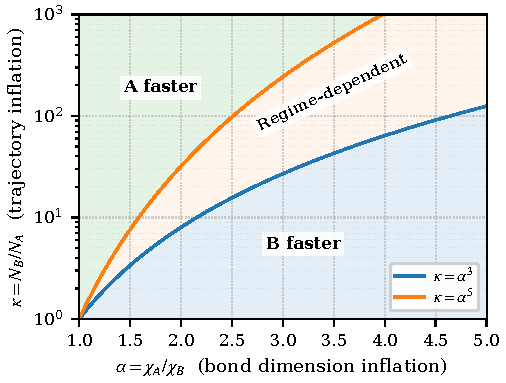
\includegraphics[width=\linewidth]{figures/ak_plot.pdf}
    \caption{
    \textbf{Analytical redistribution of computational cost between bond dimension and sampling requirements.}
    Decision geometry in the $(\alpha,\kappa)$ plane for two physically equivalent unravelings $A$ and $B$, where $\alpha=\chi_A/\chi_B$ quantifies relative per-trajectory complexity and $\kappa=N_B/N_A$ quantifies relative sampling cost.
    The curves $\kappa=\alpha^3$ and $\kappa=\alpha^5$ correspond to the decision boundaries in the thread-limited and memory-limited regimes, respectively.
    Below each curve, the reduction in per-trajectory cost associated with smaller bond dimension outweighs the increased number of trajectories; above it, the sampling overhead dominates.
    Only in the intermediate region $\alpha^3<\kappa<\alpha^5$ does the preferred unraveling depend on hardware constraints.
    }
    \label{fig:ak_plot}
\end{figure}

\subsection{Decision boundaries under realistic hardware constraints}
Quantum trajectory simulations are naturally amenable to parallel execution, since individual trajectories are statistically independent and can be evolved concurrently. To translate the abstract cost ratios $(\alpha,\kappa)$ into an end-to-end runtime comparison, we model trajectory execution on hardware with a finite parallelism budget of $p$ workers and a total memory budget $M$. These constraints determine how many of the trajectories required for a target accuracy can be evolved simultaneously and, in large-ensemble settings, whether execution is primarily limited by worker count or by memory capacity.

Let $N_j(\varepsilon)$ denote the number of trajectories required by unraveling $j$ to reach the target statistical accuracy $\varepsilon$. This is not a hardware resource, but a property of the stochastic estimator for the chosen observable and accuracy target. Let $m_j$ denote the maximum number of trajectories of unraveling $j$ that can be stored concurrently in memory, with $m_j$ scaling as
\begin{equation}
m_j \propto \frac{M}{L\, d\, \chi_j^2}.
\label{eq:mj_def}
\end{equation}
The effective parallelism for unraveling $j$ is then limited by the minimum of available workers, required trajectories, and memory capacity,
\begin{equation}
P_j = \min\!\bigl(p,\; N_j(\varepsilon),\; m_j\bigr).
\label{eq:Pj_def_cost}
\end{equation}
Using the scaling in Eq.~\eqref{eq:time_scaling_def}, the total wall time can be modeled as
\begin{equation}
T_j \propto \frac{N_j(\varepsilon)}{P_j}\,\frac{T}{\delta t}\,L\,d\,\chi_j^3,
\label{eq:Tj_cost_model}
\end{equation}
which accounts for batched concurrent execution of independent trajectories. This leads to the runtime ratio for a fixed system size and time step
\begin{equation}
\frac{T_A}{T_B}
\propto
\frac{\alpha^3}{\kappa}\,\frac{P_B}{P_A}.
\label{eq:TA_TB_cost}
\end{equation}

Equation~\eqref{eq:Pj_def_cost} also includes the fully concurrent regime in which all required trajectories fit within both the worker and memory budgets. If $N_j(\varepsilon)\le p$ and $N_j(\varepsilon)\le m_j$, then $P_j=N_j(\varepsilon)$ and all trajectories for unraveling $j$ can be executed in a single batch. In this case the required trajectory count still determines total computational work, but it no longer increases the idealized wall time. If both unravelings are fully concurrent, the wall-time comparison reduces to the per-trajectory cost ratio, $T_A/T_B\propto\alpha^3$. The hardware-dependent comparison between worker count and memory capacity becomes relevant once $N_j(\varepsilon)$ is large enough that at least one of the concurrency constraints, $p$ or $m_j$, is saturated. We therefore focus on the two large-ensemble limiting regimes that yield transparent decision boundaries.

\begin{enumerate}
\item \textbf{Thread-limited regime.}
If available workers are the bottleneck ($p \le m_A,m_B$ and $p \le N_A,N_B$), then both unravelings saturate the same parallelism, $P_A=P_B=p$, and
\begin{equation}
\frac{T_A}{T_B} \propto \frac{\alpha^3}{\kappa}.
\end{equation}
In this regime, trajectories are executed concurrently up to the worker limit, so differences in memory footprint do not affect the number of simultaneous trajectories. The competition is therefore between evolving fewer high-cost trajectories and more low-cost trajectories. Unraveling~$B$ is faster when the increase in trajectory count does not outweigh the reduction in per-trajectory cost ($\kappa < \alpha^3$), whereas unraveling~$A$ is favored when the additional sampling overhead dominates ($\kappa > \alpha^3$).

\item \textbf{Memory-limited regime.}
If memory limits concurrency ($m_A,m_B \le p$ and $m_A,m_B \le N_A,N_B$), then the number of trajectories that can be evolved in parallel is set by memory, $P_j=m_j$. Using $m_A/m_B \approx \alpha^{-2}$ yields
\begin{equation}
\frac{T_A}{T_B} \propto \frac{\alpha^5}{\kappa}.
\end{equation}
Here, the smaller bond dimension of unraveling~$B$ allows significantly more trajectories to fit in memory and be processed concurrently. In this regime, having more required trajectories is partially compensated by increased concurrency, while the larger bond dimension of unraveling~$A$ restricts the number of simultaneous trajectories. As a result, unraveling~$B$ is favored whenever $\kappa < \alpha^5$.
\end{enumerate}

The two curves $\kappa=\alpha^3$ and $\kappa=\alpha^5$ therefore define the thread-limited and memory-limited decision boundaries in the $(\alpha,\kappa)$ plane. For large-ensemble simulations in which all required trajectories cannot be executed simultaneously, these boundaries identify whether the reduction in per-trajectory cost associated with smaller bond dimension compensates the increased sampling effort. Outside the interval $\alpha^3 < \kappa < \alpha^5$, the same unraveling is favored in both limiting hardware regimes. Only within this intermediate window does the preferred unraveling depend on whether execution is closer to the thread-limited or memory-limited regime.

\begin{figure*}
    \centering
    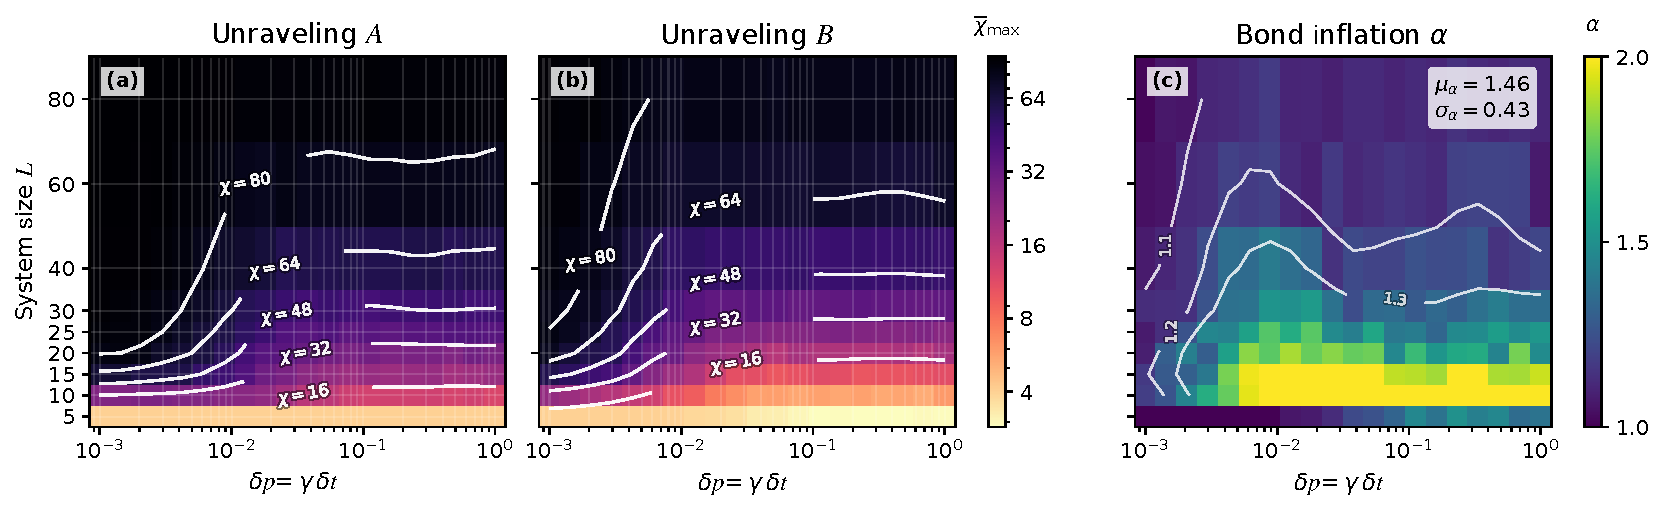
\includegraphics[width=\linewidth]{figures/large_scale_3.pdf}
    \caption{
    \textbf{Finite-size bond dimension trends in the TJM depolarizing benchmark.}
    \textbf{(a,b)} Peak average trajectory bond dimension $\overline{\chi}$ as a function of system size $L$ and discretized noise parameter $\delta p=\gamma \delta t$ for (a) Pauli-jump and (b) measurement-based unravelings. White contours denote constant $\chi_{\mathrm{max}}$.  
    \textbf{(c)} Bond inflation ratio $\alpha = \chi_{\mathrm{max},A}/\chi_{\mathrm{max},B}$ as a function of system size $L$ and $\delta p$.  
    Results are obtained for a transverse-field Ising chain initialized in a N\'eel state, evolved to $T=5$ with $\delta t=0.1$ under local depolarizing noise using the TJM update rule.
    }
    \label{fig:Large_Scale}
\end{figure*}

The decision geometry visualized in Fig.~\ref{fig:ak_plot} is analytical and independent of any particular physical model or implementation-specific pre-factors. What varies between simulation scenarios is therefore not the geometry itself, but the location of a given problem within the $(\alpha,\kappa)$ plane. Most importantly, the numerical values of $\alpha$ and $\kappa$ are \emph{not} intrinsic properties of an unraveling. They depend on physical parameters such as the Hamiltonian and noise model, as well as numerical discretization choices and system size.

A central contribution of this work is to demonstrate this regime dependence explicitly. Using large-scale benchmarks, we show that the same pair of physically equivalent unravelings can occupy qualitatively different locations in the $(\alpha,\kappa)$ plane as noise strength, time step, and system size are varied. As a result, the preferred unraveling can change across parameter regimes even though the underlying decision geometry remains fixed.
In the following sections, we extract $(\alpha,\kappa)$ for representative unravelings across a range of physical and numerical regimes. This allows us to place concrete simulation scenarios within the $(\alpha,\kappa)$ plane and to identify when apparent cost reductions in one channel are offset by increases in another.

\section{Benchmarking cost redistribution}
\label{sec:benchmarking}

\subsection{Setup}

We now turn to a concrete case study in which we extract the bond dimension and sampling inflation factors $(\alpha,\kappa)$ for representative stochastic unravelings under controlled physical and numerical conditions. The goal of this section is not to identify model-specific phenomena, but to empirically demonstrate how $\alpha$ and $\kappa$ vary with algorithmic and physical parameters, and how this variation reshapes the cost trade-offs identified in Sec.~\ref{sec:cost_structure}.

The main benchmarks in this section are performed on the one-dimensional transverse-field Ising model with open boundary conditions
\begin{equation}
H = -J \sum_{i=1}^{L-1} Z_i Z_{i+1} \;-\; g \sum_{i=1}^{L} X_i ,
\end{equation}
with parameters fixed to the critical point $J=g=1$. Simulations are initialized in the N\'eel product state vector
\begin{equation}
\ket{\psi_0} = \ket{0,1,0,1\cdots},
\end{equation}
which rapidly generates entanglement under coherent dynamics while avoiding symmetries that could artificially simplify the evolution.
While we focus on this specific model, the cost-redistribution mechanisms identified below arise from trajectory-level bond growth, sampling variance, and discretization choices rather than from the detailed physics of this model alone.

For the main transverse-field Ising benchmarks, we consider open-system dynamics generated by local depolarizing noise implemented via local jump operators. To isolate the algorithmic consequences of different stochastic representations of the same Lindblad generator, we compare two physically equivalent unravelings:
\begin{enumerate}
    \item \textbf{Pauli-jump unraveling (A).}  
    Each site undergoes stochastic quantum jumps generated directly by the Pauli operators $X$, $Y$, and $Z$. This corresponds to the standard depolarizing channel and produces relatively infrequent but strong state updates.

    \item \textbf{Measurement-based unraveling (B).}  
    The same depolarizing channel is decomposed into projective measurement outcomes, e.g., $\{\ket{0}\!\bra{0}, \ket{1}\!\bra{1}\}$ for $Z$, $\{\ket{+}\!\bra{+}, \ket{-}\!\bra{-}\}$ for $X$, and $\{\ket{+_i}\!\bra{+_i}, \ket{-_i}\!\bra{-_i}\}$ for $Y$. This yields more frequent but weaker stochastic updates, modifying individual trajectory dynamics while reproducing the same Lindblad evolution upon ensemble averaging. To ensure equivalence of the underlying master equation under this decomposition, the corresponding rates satisfy $\gamma_B = 2\gamma_A=:2\gamma$.
\end{enumerate}

These two unravelings are not intended to be exhaustive. Other stochastic representations of Lindblad dynamics have been explored in prior work and can give rise to qualitatively different trajectory statistics and convergence behavior~\cite{vovk_2022, vovk_2024, SimonSimulation, AnalogSimQuantinuum}. Our objective here is not to rank all possible unravelings, but to use a minimal pair to expose mechanisms by which algorithmic choices redistribute computational cost in MPS-based trajectory simulations. Unless stated otherwise, the benchmarks in this section use local depolarizing noise. Other noise models are considered later as additional case studies and may shift the extracted $(\alpha,\kappa)$ values while leaving the analytical decision geometry unchanged. Finally, this comparison can be generalized to more than two unravelings.

All simulations are performed using the \emph{tensor jump method} (TJM) \cite{sander_TJM_2025}. No explicit maximum bond dimension is imposed, so unitary evolution is performed using two-site TDVP without a hard cutoff on $\chi$. Instead, bond growth is controlled through a discarded-weight truncation criterion, i.e., after each two-site update, singular values are truncated using a threshold of $s_\text{max}=10^{-6}$. The bond dimension therefore adapts dynamically in response to both coherent evolution and stochastic jumps.

Expectation values are obtained by averaging over stochastic trajectories. In the ideal limit of infinite trajectory number, converged time step, and controlled MPS truncation, both valid unravelings reproduce the same Lindblad expectation values. At finite numerical resources, however, the two unravelings can differ in trajectory bond dimension, estimator variance, and therefore total computational cost.

Throughout this work, fixed accuracy means convergence with respect to the numerical controls relevant for the comparison. We distinguish three contributions. First, time-step error is controlled by choosing $\delta t$ within the convergent regime of the TJM scheme and, where needed, checking stability under decreasing $\delta t$. Second, MPS projection and truncation errors are controlled by the discarded-weight threshold and are assumed to be subdominant for the reported comparisons. Third, sampling error is estimated from trajectory-to-trajectory fluctuations of the measured observables. For an observable $O$ and unraveling $U$, this gives a standard error of the mean of
\begin{equation}
\Delta O_U \approx \frac{\sigma_U[O]}{\sqrt{N}},
\end{equation}
where $\sigma_U[O]$ is the empirical standard deviation across trajectories. For large systems, where exact reference evolution is unavailable, this statistical error is an estimator uncertainty rather than a directly measured absolute error to the exact Lindblad solution. In the small-system convergence benchmarks below, exact reference evolution is available, and we additionally use the absolute deviation from the exact result to extract trajectory counts at a prescribed accuracy.

All benchmarks are performed using \textsc{MQT-YAQS}~\cite{YAQS, wille_mqt2024}, our MPS-based framework for stochastic and time-dependent quantum simulation. Results are obtained on a desktop equipped with an Intel Core i7-13600KF CPU with 20 threads and 64 GB of RAM. Within each comparison, identical build settings, linear algebra backends, and threading configurations are used to ensure that observed differences reflect algorithmic behavior rather than environment-dependent performance artifacts. Unless otherwise specified, bond dimensions are reported as the maximum bond dimension reached over the course of the evolution.

\begin{figure*}
    \centering
  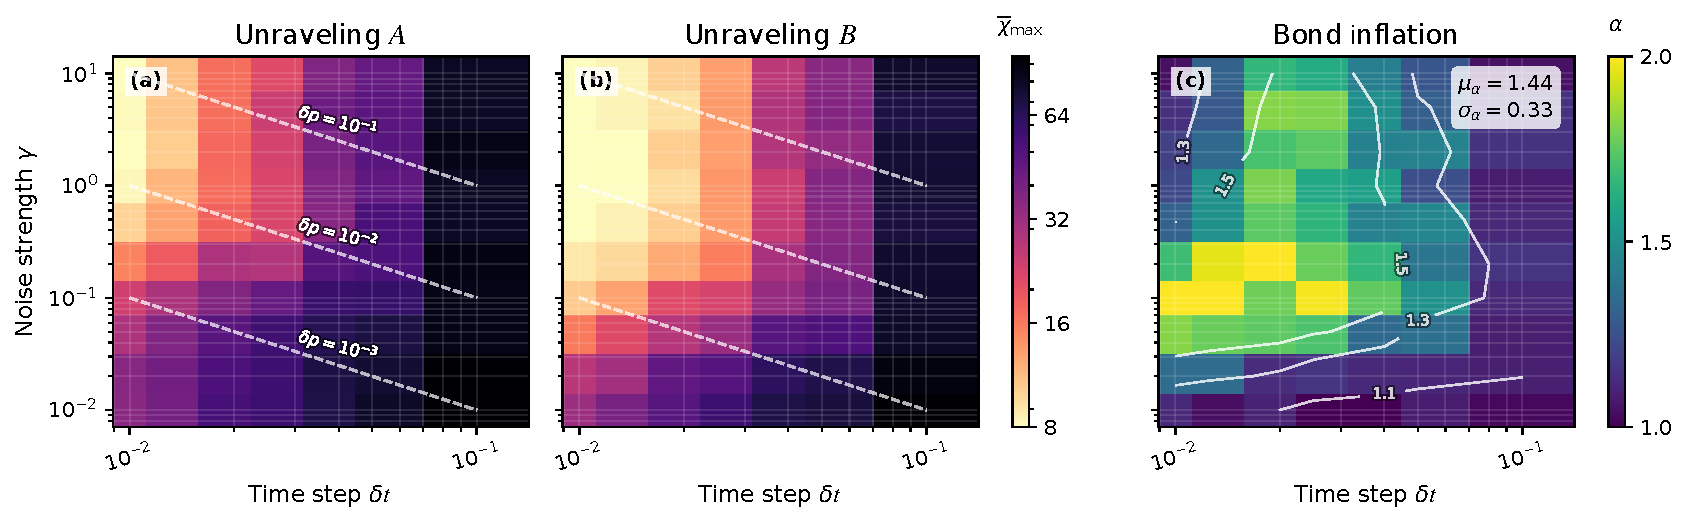
\includegraphics[width=\linewidth]{figures/gamma_dt_2.pdf}
    \caption{
    \textbf{Monitoring-resolution dependence of bond dimension in $(\gamma,\delta t)$ space.}
    \textbf{(a,b)} Peak trajectory bond dimension $\chi$ for $L=65$ as a function of noise strength $\gamma$ and time step $\delta t$ for unravelings A and B. Dashed lines indicate contours of constant $\delta p=\gamma\delta t$.
    \textbf{(c)} Bond inflation ratio $\alpha=\chi_A/\chi_B$ as a function of $\gamma$ and $\delta t$.
    Results are shown up to $T=5$ using $N=30$ trajectories to characterize systematic bond dimension trends.
    }
    \label{fig:gamma_dt}
\end{figure*}

\begin{figure}
    \centering
  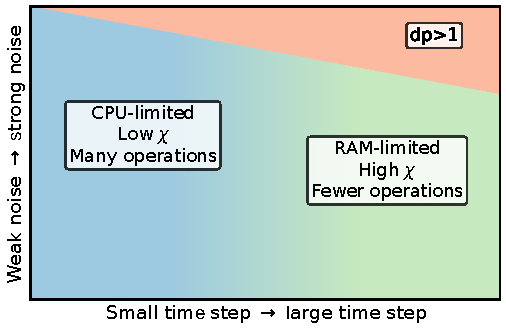
\includegraphics[width=.9\linewidth]{figures/gamma_dt_summary_2.pdf}
    \caption{
    \textbf{Schematic discretization-controlled computational regimes.}
    Conceptual map in $(\gamma,\delta t)$ space summarizing the behavior in \cref{fig:gamma_dt}. 
    For small $\delta t$, fine monitoring suppresses trajectory bond dimension $\chi$ but increases the number of updates required to reach fixed physical time. 
    For larger $\delta t$, bond dimension becomes weakly-dependent on $\gamma$ and memory usage dominates resource requirements. 
    Boundaries are schematic and indicate smooth crossovers rather than sharp transitions.
    }
    \label{fig:gamma_dt_summary}
\end{figure}

\subsection{Finite-size trends of trajectory bond dimension}
A common intuition in open-system simulation is that environmental noise suppresses entanglement and thereby reduces the bond dimension required to represent quantum states. In trajectory-based methods, this expectation is often transferred to the entanglement of individual stochastic trajectories, suggesting that stronger noise may reduce the cost of MPS-based simulations. Here we test this intuition within the present TJM/MCWF-style benchmark by resolving the trajectory-level maximum bond dimension $\chi_{\mathrm{max}}$ as a function of system size $L$. This quantity directly controls the per-trajectory memory footprint and contributes to the per-trajectory runtime cost.

All results in this subsection are obtained for fixed physical evolution time $T=5$ and time step $\delta t=0.1$, using $N=30$ stochastic trajectories. While this trajectory count is insufficient for fully converged observables, it captures systematic finite-size trends in $\chi$ as a function of $L$ and noise strength. Increasing $N$ reduces statistical fluctuations in these estimates but does not change the benchmark role of this subsection, which is to characterize the bond dimension component of the cost model.

\cref{fig:Large_Scale}\textbf{(a,b)} shows the trajectory-averaged peak bond dimension $\overline{\chi}$ as a function of system size $L$ and effective jump probability $\delta p=\gamma\delta t$ for two physically equivalent unravelings. We fix $\delta t$ and vary the physical noise strength $\gamma$, thereby isolating how trajectory complexity responds to increasing stochasticity at fixed numerical resolution. Although the continuous-time Lindblad limit formally requires small per-step jump probabilities, we also include larger values of $\delta p$ as an algorithmic probe of stochastic update strength. For sufficiently large $\delta p$, the discrete-time dynamics no longer represents a strict continuous-time unraveling without resolving multiple jumps per time step, and these points should therefore be interpreted only as a probe of the implemented update rule.

At small and intermediate system sizes, increasing $\delta p$ reduces $\overline{\chi}$ for both unravelings, consistent with the standard intuition that stochastic jumps interrupt coherent entanglement growth along individual trajectories. The more relevant feature of \cref{fig:Large_Scale}, however, is the finite-size behavior of this reduction. Over the accessible finite-time system-size range, the noise-induced suppression of bond dimension becomes progressively less pronounced as $L$ increases, and $\overline{\chi}$ approaches a plateau-like regime that depends only weakly on $\delta p$ for the parameters studied here.

This plateau-like behavior should be interpreted as a benchmark-specific finite-size trend rather than as an asymptotic statement about arbitrary MPS trajectory methods. In particular, the behavior reported here is tied to the TJM/MCWF-style update structure, the finite evolution time, the transverse-field Ising dynamics considered, and the two unravelings compared. The low-noise dynamics already exhibits limited bond growth over the accessible range, so part of the apparent saturation may reflect the finite-time entanglement structure of the underlying model rather than a universal limitation imposed by trajectory sampling. Other trajectory constructions, including Kraus- or reset-based representations, may therefore produce qualitatively different finite-size behavior and can in some limits drive trajectories closer to product-state structure.

The quantitative contrast between unravelings is summarized in \cref{fig:Large_Scale}\textbf{(c)}, which shows the bond inflation ratio $\alpha = \chi_A/\chi_B$. Moderate inflation ($\alpha \sim 1.2$--$1.5$) appears at intermediate system sizes and noise strengths, indicating that unraveling choice can meaningfully affect per-trajectory memory cost in this regime. As $L$ increases, $\alpha$ narrows toward unity in the present benchmark. Since $\alpha$ is a relative comparison between the two specified unravelings, this narrowing should not be read as an absolute statement that unraveling choice becomes irrelevant in all large systems. Rather, it reflects the plateau-like bond dimension behavior observed for this finite-time benchmark and the particular TJM update rule used here.

These results show that reduced trajectory bond dimension at small and intermediate system sizes does not automatically imply a persistent reduction in per-trajectory cost across the accessible system-size range. More generally, they illustrate why bond dimension alone is not sufficient to assess the total cost of a trajectory simulation. Even when noise suppresses trajectory entanglement, the magnitude and persistence of this reduction depend on the stochastic representation, numerical resolution, and finite-time entanglement structure of the simulated model.

Finally, although \cref{fig:Large_Scale} parametrizes noise via $\delta p=\gamma\delta t$, the present analysis isolates only the bond dimension component of computational cost. Total runtime additionally depends on trajectory sampling requirements, quantified by $\kappa$. We therefore turn next to extracting the joint $(\alpha,\kappa)$ characterization across parameter regimes.

\begin{figure*}
    \centering
  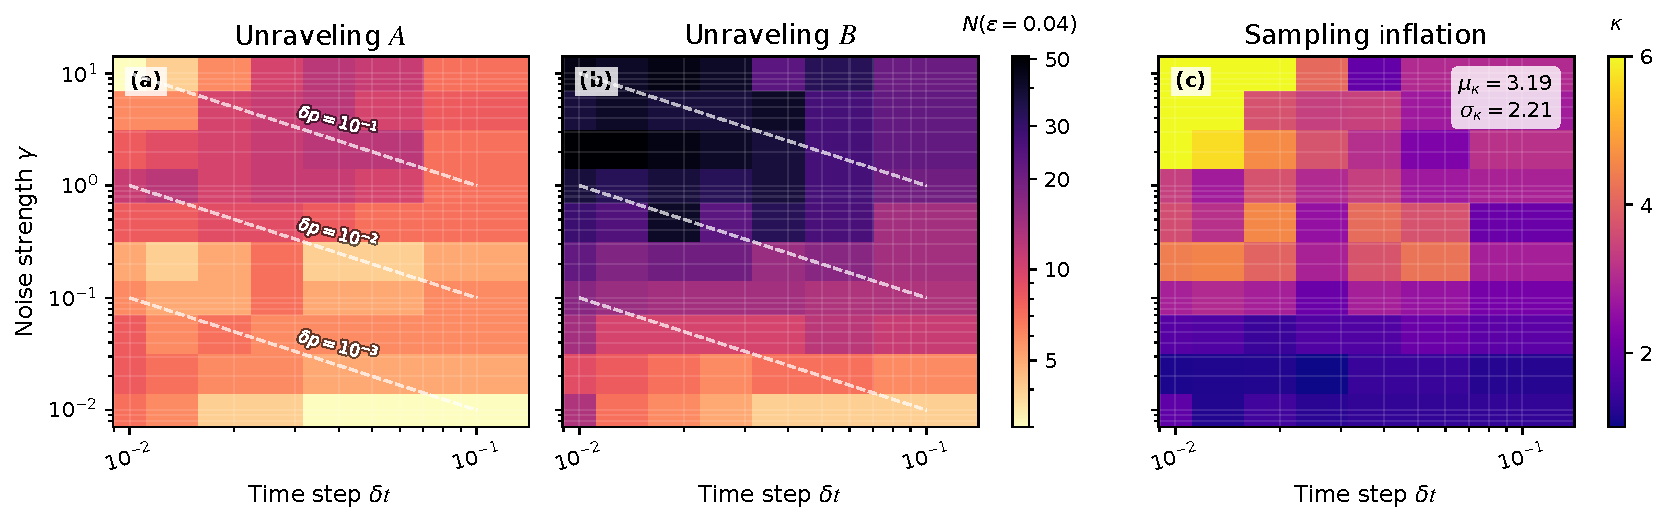
\includegraphics[width=\linewidth]{figures/convergence_2.pdf}
    \caption{
    \textbf{Sampling requirements in a small-system exact-reference benchmark.}
    \textbf{(a,b)} Number of trajectories $N(\varepsilon=0.04)$ required for the trajectory-averaged correlator $\langle X_4 X_{5} \rangle$ to reach a fixed absolute deviation from exact reference evolution, shown as functions of noise strength $\gamma$ and time step $\delta t$ for a 10-site system evolved to $T=2$. Dashed contours indicate constant $\delta p=\gamma\delta t$.  
    \textbf{(c)} Sampling inflation factor $\kappa = N_B/N_A$, quantifying the relative trajectory count required by unravelings A and B to reach the same reference-accuracy threshold. Because exact evolution is available for this small system, the extracted trajectory counts measure absolute error relative to the Lindblad reference; for large systems, the corresponding sampling cost is estimated from trajectory-to-trajectory variance through the standard error of the mean.
    }
    \label{fig:convergence}
\end{figure*}

\subsection{Trade-offs within individual trajectories}
The previous section showed that, for the TJM benchmark and unravelings considered, the observed bond dimension reduction becomes less pronounced over the accessible finite-time system-size range. We now fix the system size in this plateau-like regime and examine how trajectory-level complexity depends on the interplay between physical noise strength $\gamma$ and numerical time-step resolution $\delta t$.

Throughout this subsection we restrict to time steps $\delta t \le 0.1$, for which the tensor jump method is provably convergent and achieves fixed-accuracy error scaling of $\mathcal{O}(\delta t^3)$~\cite{sander_TJM_2025}. This ensures that the observed trends reflect controlled algorithmic trade-offs rather than uncontrolled time-discretization errors.

The effective jump probability per time step, $\delta p=\gamma\delta t$, is often used as a compact descriptor of stochasticity. However, it combines two distinct controls: the physical noise strength $\gamma$ and the numerical resolution $\delta t$ at which stochastic events are sampled. Fixing $\delta p$ therefore does not uniquely specify how Lindblad dynamics is resolved along individual trajectories.

\cref{fig:gamma_dt} disentangles these effects by resolving the maximum bond dimension $\chi$ as a function of $(\gamma,\delta t)$ for two physically equivalent unravelings. Dashed contours indicate lines of constant $\delta p$. All results are shown at fixed system size $L=65$ and final time $T=5$, where \cref{fig:Large_Scale} indicates that the finite-time bond dimension trends have entered the plateau-like regime.

At fixed physical noise strength $\gamma$, decreasing the time step $\delta t$ systematically reduces $\chi$ for both unravelings. Finer temporal resolution distributes stochastic events more evenly in time, interrupting coherent entanglement growth and suppressing bond dimension accumulation. Along contours of constant $\delta p$, however, $\chi$ still varies substantially with $\delta t$, showing that jump probability alone does not determine trajectory-level entanglement complexity. Coarser time steps sample stochastic events less frequently, allowing coherent evolution to generate larger bond dimensions even when $\delta p$ is held fixed.

The two unravelings exhibit systematic quantitative differences across the $(\gamma,\delta t)$ plane, summarized by the bond inflation factor $\alpha=\chi_A/\chi_B$ in \cref{fig:gamma_dt}(c). Enhanced inflation, $\alpha\sim1.5$--$2.0$, appears at intermediate noise strengths and fine time steps, where coherent entanglement growth competes with weak monitoring. By contrast, $\alpha$ approaches unity both in the strongly monitored fine-time-step regime and in the coarse-time-step regime, although for different reasons: in the former case, entanglement is rapidly suppressed for both unravelings, while in the latter stochastic events are too coarsely resolved to generate large unraveling-dependent differences.

These results show that discretization reshapes trajectory-level entanglement growth without changing the underlying Lindblad generator. Within the cost framework of Sec.~\ref{sec:cost_structure}, the resulting shifts in bond dimension define the parameter-dependent inflation factor $\alpha(\gamma,\delta t)$. Bond inflation alone, however, does not determine total simulation cost; trajectory sampling requirements introduce an additional trade-off, captured by the sampling inflation factor $\kappa$.

\subsection{Sampling inflation at fixed physical accuracy}
\label{sec:sampling_inflation}

The previous sections characterized how physical and numerical choices reshape the bond dimension of individual trajectories and thereby determine the bond inflation factor $\alpha$. Total simulation cost, however, is governed by ensemble averages and therefore also depends on trajectory-to-trajectory fluctuations. We now quantify this second cost channel by extracting the sampling inflation factor $\kappa$ from exact benchmarks.

\cref{fig:convergence} shows the 
number of trajectories required to reach a fixed absolute error threshold $\epsilon\leq0.04$ across the full time evolution in the central bond correlator $\langle X_4 X_{5} \rangle$ for a 10-site system evolved exactly to $T=2$. The small system size permits exact reference evolution, ensuring that the extracted trajectory counts isolate statistical error rather than truncation or discretization effects.

Both unravelings exhibit standard Monte Carlo convergence, $\varepsilon \propto {1}/{\sqrt{N}}$, indicating identical asymptotic scaling. The error pre-factors, however, depend strongly on $(\gamma,\delta t)$ and differ substantially between unravelings. These pre-factor differences define the sampling inflation factor $\kappa(\varepsilon)$ introduced in Eq.~\eqref{eq:alpha_kappa_def}.

The resulting $\kappa(\gamma,\delta t)$ map in \cref{fig:convergence}\textbf{(c)} displays broad variation across parameter space, with regions where one unraveling requires several times more trajectories than the other to achieve identical accuracy. Notably, the structure of $\kappa$ does not mirror that of the bond inflation factor $\alpha$: parameter regions with reduced bond dimension can exhibit enhanced sampling requirements, and vice versa. Sampling inflation therefore constitutes an independent cost channel that cannot be inferred from trajectory entanglement alone.

Together $\alpha(\gamma,\delta t)$ and $\kappa(\gamma,\delta t)$ quantify two distinct forms of cost redistribution: entanglement inflation within trajectories and variance inflation across trajectories. In the next section, we combine these empirically extracted inflation factors with hardware constraints to guide simulation design.

\section{Generalized cost extraction and hardware projections}
\label{sec:generalized_framework}

We now turn the preceding cost analysis into a practical workflow. Given two physically equivalent unravelings of the same Lindblad dynamics, the goal is to estimate the bond dimension and sampling inflation factors $(\alpha,\kappa)$ from modest pilot simulations and use them to predict which unraveling is favored under specified memory and parallelism constraints.

We first describe the extraction protocol and then apply it to a Heisenberg-chain benchmark with depolarizing, dephasing, and bit-flip noise. This yields concrete hardware-aware decision maps illustrating how different noise channels populate the cost plane.

\subsection{Protocol for extracting inflation factors}
\label{sec:extraction_protocol}
We consider two physically equivalent unravelings, $A$ and $B$, of the same Lindblad generator. The objective is to determine the bond dimension inflation ratio $\alpha$ and the sampling inflation ratio $\kappa$ for a fixed simulation scenario.

The inflation factors $(\alpha,\kappa)$ are scenario-dependent quantities. 
For a fixed Hamiltonian, noise model, time step $\delta t$, final time $T$, initial state, observable, and target statistical accuracy $\epsilon_{\mathrm{target}}$, they quantify how two physically equivalent unravelings redistribute computational cost.
All quantities must therefore be evaluated under identical physical and numerical conditions.

For each unraveling $j\in\{A,B\}$, we perform a pilot trajectory simulation with a moderate number of trajectories $N_{\mathrm{pilot}}$ and extract the maximum bond dimension $\chi_j$ reached during evolution. Their ratio defines $\alpha$ for this simulation scenario.

To quantify sampling effort, we evaluate the variance of the chosen observable across trajectories at the target time. 
Let $\sigma_j$ denote the empirical standard deviation of unraveling $j$. 
For a target standard error $\epsilon_{\mathrm{target}}$, the required trajectory count follows from the central limit theorem as
\begin{equation}
N_j \approx \left(\frac{\sigma_j}{\epsilon_{\mathrm{target}}}\right)^2.
\end{equation} 
The corresponding ratio $N_B/N_A$ defines $\kappa$.

Importantly, the extraction requires only modest pilot simulations and avoids exhaustive convergence studies. 
Once determined, these inflation factors can be inserted into the hardware-aware cost model of ~\cref{sec:cost_structure} to estimate runtime behavior under arbitrary memory and parallelism constraints.
The inflation factors are scenario-dependent but dimensionless. Once extracted, they can be used for hardware projections within the same algorithmic regime, provided the relevant bond dimension and variance trends remain comparable.

\begin{figure}
    \centering
    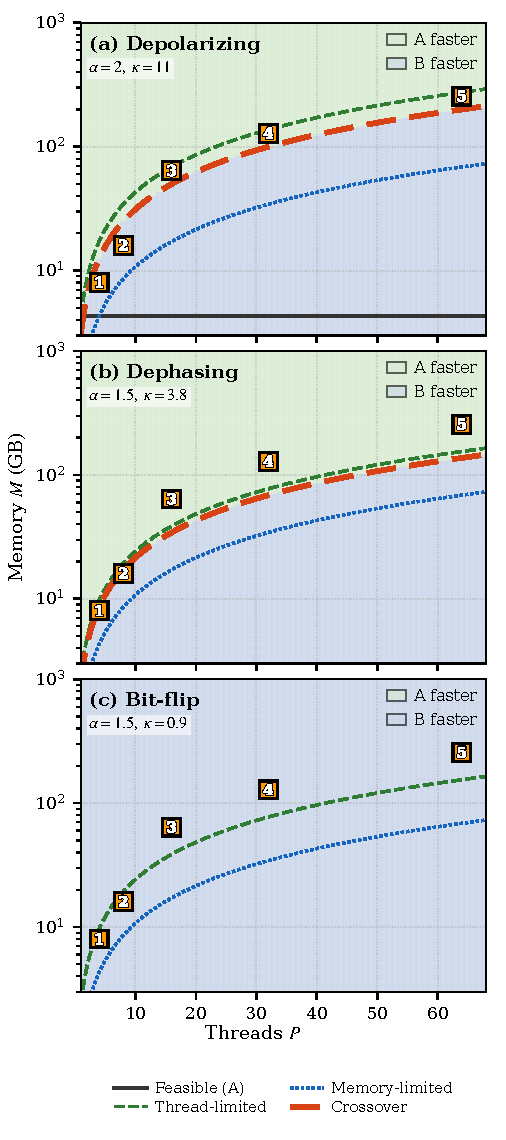
\includegraphics[width=\linewidth]{figures/mp_triptych.pdf}
    \caption{
    \textbf{Hardware-aware decision maps for Heisenberg noise channels.}
    Runtime-minimizing regions in the plane of physical memory $M$ (GB) and available workers $P$ for
    (a) depolarizing $(\alpha,\kappa)=(2.0,11)$,
    (b) dephasing $(1.5,3.8)$,
    and (c) bit-flip $(1.5,0.9)$ noise.
    Green (blue) shading indicates where unraveling $A$ ($B$) yields lower modeled runtime.
    Solid, dashed, and dotted lines denote the feasibility threshold and memory/thread-limited boundaries, while the dash-dotted line marks the crossover $T_A=T_B$.
    Markers (1–5) represent representative hardware classes from 8 GB/4 threads to 256 GB/64 threads.
    Memory is referenced to $M_B=L\chi_B^2\times16$ bytes with $L=1024$ and $\chi_B=256$.
    }
    \label{fig:mp_triptych}
\end{figure}

\subsection{Hardware-aware decision maps}
\label{sec:heisenberg_hardware}
To translate the extracted inflation factors into hardware-aware runtime estimates, we project each scenario onto the hardware-aware decision geometry derived in ~\cref{sec:cost_structure}. The decision maps in \cref{fig:mp_triptych} are constructed from the inflation factors 
extracted for the Heisenberg chain with $L=16$, couplings $J=h=1$, noise strength $\gamma=0.1$, time step $\delta t=0.1$, and final time $T=2$. The observable is a local $Z$ expectation value, and trajectory counts are estimated to reach a target standard error $\epsilon_{\mathrm{target}}=0.01$ using $N_{\mathrm{pilot}}=100$ pilot trajectories. Pilot trajectory counts were chosen to give stable estimates of the bond dimension and variance trends used in the projection.

We consider three noise models, depolarizing ($X$, $Y$, $Z$ jumps), dephasing ($Z$), and bit-flip ($X$). The Pauli jumps are unraveling A and their measurement-based analogs are unraveling B as done in \cref{sec:benchmarking}.
The resulting $(\alpha,\kappa)$ values are therefore scenario-specific and serve here as concrete inputs to the hardware projection.

We adopt a common reference configuration corresponding to a large-scale simulation with $L=1024$ and $\chi_B=256$. Assuming 16 bytes per complex number and unit implementation overhead, the baseline memory per trajectory of unraveling $B$ is
\begin{equation}
M_B = L\,\chi_B^2 \times 16~\mathrm{bytes}.
\end{equation}

For fixed $(\alpha,\kappa)$, the modeled runtime ratio
\begin{equation}
\frac{T_A}{T_B} \sim \frac{\alpha^3}{\kappa}\,\frac{P_B}{P_A}
\end{equation}
induces a partition of the $(M,P)$ plane into regions where either unraveling~$A$ or $B$ has lower modeled runtime. Each panel of \cref{fig:mp_triptych} displays this decision map for one of the Heisenberg noise channels.
The solid line marks the feasibility threshold $M=\alpha^2 M_B$, dashed and dotted lines denote the onset of thread- and memory-limited execution, and the dash-dotted line indicates the crossover $T_A=T_B$ when present.

To anchor the maps to realistic computational regimes, we overlay representative hardware configurations corresponding approximately to:
\begin{enumerate}
    \item embedded or edge devices ($M\sim8$~GB, $P\sim4$),
    \item laptops ($M\sim16$~GB, $P\sim8$),
    \item desktops ($M\sim64$~GB, $P\sim16$),
    \item small servers ($M\sim128$~GB, $P\sim32$),
    \item HPC nodes ($M\sim256$~GB, $P\sim64$).
\end{enumerate}
These markers illustrate how identical physical simulations may favor different unravelings depending on available memory and parallelism.

The three noise channels therefore occupy distinct regions of the hardware decision geometry. Depolarizing noise, with $(\alpha,\kappa)=(2.0,11)$, lies deep in the trade-off regime such that the crossover occurs near the onset of thread saturation, so modest changes in memory or worker count can reverse the preferred unraveling. Dephasing noise, $(1.5,3.8)$, remains in the trade-off quadrant but shifts the crossover toward lower memory, enlarging the region where reduced bond dimension compensates sampling overhead.
In contrast, bit-flip noise, $(\alpha,\kappa)=(1.5,0.9)$, satisfies $\alpha>1$ and $\kappa<1$, so unraveling~$B$ has both lower per-trajectory complexity and lower sampling cost and therefore enters the strict-dominance regime.

Altogether, these cases illustrate that the analytical decision geometry is general, but the practical unraveling choice depends sensitively on how a 
given physical simulation populates the $(\alpha,\kappa)$ plane.

The runtime model should be interpreted as a resource-level decision criterion rather than a calibrated wall-clock predictor. The equations retain the dominant dependence on bond dimension, trajectory count, memory, and parallelism, while omitting implementation-dependent prefactors from batching, scheduling, local tensor kernels, linear-algebra backends, and communication overhead. Such prefactors can be important whenever fixed overheads are comparable to the MPS evolution time. The purpose of the hardware projections is therefore not to predict absolute runtimes, but to identify when reduced per-trajectory complexity is expected to compensate, or fail to compensate, increased sampling effort. Quantitative wall-clock optimization for a specific code path or architecture would require an additional implementation-level calibration.


\section{Unifying interpretation and outlook}
This work develops a resource-level view of MPS-based quantum trajectory simulations. By separating memory, runtime, and sampling costs, we show that trajectory entanglement or bond dimension alone is not sufficient to predict end-to-end simulation cost. The inflation factors $(\alpha,\kappa)$ provide a compact way to compare physically equivalent unravelings by combining per-trajectory complexity with statistical sampling requirements under finite memory and parallelism.

A central outcome is that reduced trajectory bond dimension does not automatically imply reduced total cost. In the TJM/MCWF-style benchmarks studied here, environmental noise can suppress trajectory entanglement in some regimes, but this reduction can weaken over the accessible finite-time system-size range or require finer time-step resolution. In addition, an unraveling with lower per-trajectory complexity can require more trajectories to reach the same statistical accuracy. Bond dimension is therefore a useful diagnostic, but not a standalone complexity measure once discretization, truncation, and sampling are taken into account.

We also introduced a practical protocol for extracting bond dimension and sampling inflations from modest pilot simulations. Applying this protocol to Heisenberg-chain benchmarks with different noise channels shows that distinct physical settings can occupy different regions of the $(\alpha,\kappa)$ plane, including both trade-off and strict-dominance regimes. The decision geometry is general, but the extracted values depend on the model, observable, target accuracy, and simulation strategy.

The resulting hardware decision maps make unraveling choice an explicitly resource-dependent algorithmic decision. Physically equivalent stochastic representations may be favored or disfavored depending on memory capacity, available parallelism, time-step resolution, and sampling variance. Thus, the preferred unraveling is not an intrinsic property of the Lindblad dynamics alone, but emerges from the full computational setting.

The scope of this work is deliberately limited to exposing these cost channels rather than exhaustively optimizing over all stochastic representations. Other trajectory constructions may lead to different values of $(\alpha,\kappa)$ or different bond dimension behavior. This reinforces the main point: meaningful assessment of noisy quantum simulation requires explicit resource accounting. No single quantity, such as bond dimension, time step, noise strength, or trajectory count, provides a universal complexity measure. Instead, simulation strategies should be evaluated by how computational cost is distributed across representation, sampling, and hardware resources.
It is the 
hope that this work can contribute providing a powerful machinery of classically simulating large-scale quantum systems and at the same time help turning quantum simulators into quantifiable quantum technological devices.

\section*{Acknowledgments}
This work has been supported by the Munich Quantum Valley, which is supported by the Bavarian state government with funds from the Hightech Agenda Bayern Plus (for which this work is the result of a collaboration 
of two nodes). It has also been supported by the Clusters of Excellence MATH+ 
and ML4Q. It has additionally received funds from
the European Union under the Horizon Europe Programme as part of the European Research Council projects DA QC (Grant Agreement 101001318) and DebuQC (Grant Agreement 101030988),
as well as Berlin Quantum (for which this work reflects joint work now involving the Weierstrass Institute Berlin). It has also received funding from the BMFTR (MuniQC-Atoms), the DFG (CRC 183, SPP 2514), and the Quantum Flagship (PasQuans2, Millenion). For MATH+, Millenion, SPP 2514, and the Munich Quantum Valley, this work is the result of a collaboration involving more than one node each.

\bibliographystyle{apsrev4-2}
\bibliography{bib.bib}

\end{document}
